\documentclass[xcolor=table]{beamer}
\usepackage[utf8]{inputenc}
\usepackage{default}
\usepackage{xspace,setspace}
\usepackage{amsmath,amsthm,amssymb}
\usepackage{ellipsis}
\usepackage[pdftex]{epsfig}
\usepackage{listliketab}
\usepackage[table]{xcolor}
\usepackage{booktabs}
\usepackage{amsmath}

\usepackage{pgf}
\usepackage{tikz}
\usetikzlibrary{arrows,automata}
\usetikzlibrary{graphs}
\tikzset{
     mainNode/.style =
        { circle
        , draw
        %, fill=blue!20,
        %, font=\sffamily\Large\bfseries
        }
}

\usetheme{AnnArbor}
%\usetheme{Berlin}
%\usetheme{Bergen}
%\usetheme{Antibes}
%\usetheme{Goettingen}
%\usetheme{Warsaw}
%\usetheme{Darmstadt}
%\usetheme{JuanLesPins}
%\setbeamertemplate{navigation symbols}{}
%\usecolortheme{beaver}
%\usecolortheme{rose}
%\usecolortheme{seagull}
%\usecolortheme{dove}
%\usecolortheme{seahorse}
%\usecolortheme{crane}
%\usepackage{color,colortbl}
%\usepackage{texnansi}
%\usepackage{marvosym}
%\usepackage{comment}


%\setbeamertemplate{frametitle}
%{\begin{centering}\smallskip
%   \insertframetitle\par
%   \smallskip\end{centering}}
%\setbeamertemplate{itemize item}{$\bullet$}
%\setbeamertemplate{navigation symbols}{}
%\setbeamertemplate{footline}[text line]{%
%    \hfill\strut{%
%        \scriptsize\sf\color{black!60}%
%        \quad\insertframenumber
%    }%
%    \hfill
%}

% Define some colors:

\definecolor{DarkFern}{HTML}{407428}
\definecolor{DarkCharcoal}{HTML}{4D4944}
\colorlet{Fern}{DarkFern!85!white}
\colorlet{Charcoal}{DarkCharcoal!85!white}
\colorlet{LightCharcoal}{Charcoal!50!white}
\colorlet{AlertColor}{orange!80!black}
\colorlet{DarkRed}{red!70!black}
\colorlet{DarkBlue}{olive!70!black}
\colorlet{DarkGreen}{green!70!black}
\definecolor{brickred}{RGB}{132,31,39}

% Use the colors:

%\setbeamercolor{title}{fg=Fern}
%\setbeamercolor{frametitle}{fg=Fern}
%\setbeamercolor{section title}{fg=Fern}
%\setbeamercolor{section in toc}{fg=Fern}
%\setbeamercolor{section name}{fg=Fern}
%\setbeamercolor{section in head/foot}{fg=Fern}
%\setbeamercolor{subsection title}{fg=Fern}
%\setbeamercolor{author}{fg=Fern}
%\setbeamercolor{normal text}{fg=Charcoal}
%\setbeamercolor{block title}{fg=black,bg=Fern!25!white}
%\setbeamercolor{block body}{fg=black,bg=Fern!25!white}
%\setbeamercolor{alerted text}{fg=AlertColor}
%\setbeamercolor{itemize item}{fg=Charcoal}

%\definecolor{bottomcolour}{rgb}{0.32,0.3,0.38}
%\definecolor{middlecolour}{rgb}{0.08,0.08,0.16}
\definecolor{tcsyellow}{RGB}{253,255,102}
\definecolor{tcsolive}{RGB}{77,147,191}
\definecolor{tcsolivemedium}{RGB}{147,177,210}
\definecolor{tcsolivelight}{RGB}{235,239,252}

\definecolor{skyolive}{rgb}{0.2,0.6,1}
\definecolor{darkolive}{rgb}{0.1,0.1,0.6}
\definecolor{darkred}{rgb}{1,0.2,0.1}
\definecolor{darkgreen}{rgb}{0.5,0.8,0.4}
\definecolor{Olive}{rgb}{0,0.3,0}
\definecolor{seagreen}{rgb}{0.3,0.9,0.6}
\definecolor{olive}{cmyk}{0.8,0.1,0.95,0.40}
\definecolor{golden}{cmyk}{0.0,0.25,0.85,0.15}
\definecolor{darkgolden}{cmyk}{0.0,0.27,0.94,0.07}
\definecolor{orange}{cmyk}{0.0,0.35,1.0,0.07}
\definecolor{orange2}{cmyk}{0.0,0.6,1.0, 0.0}
\definecolor{pecan}{cmyk}{0.0,0.37,0.80,0.12}
\definecolor{cadmium}{cmyk}{0.0,0.40,0.93,0.00}
\definecolor{snake}{cmyk}{0.8,0.1,0.95,0.60}
\definecolor{tcsyellow}{RGB}{253,255,102}
\definecolor{tcsolive}{RGB}{77,147,191}
\definecolor{tcsolivemedium}{RGB}{147,177,210}
\definecolor{tcsolivelight}{RGB}{235,239,252}

\definecolor{LRed}{rgb}{1,.8,.8}
\definecolor{MRed}{rgb}{1,.6,.6}
\definecolor{HRed}{rgb}{1,.2,.2}

\newtheorem{defn}{Definition}
\newtheorem{asf}{ASF Inputs}
\newtheorem{claim}{Claim}

\setbeamercolor{item projected}{bg=darkred}
\setbeamertemplate{enumerate items}[orange2]
\setbeamercolor{frametitle}{fg=white,bg=orange2}
\setbeamercolor{title}{fg=white,bg=orange2}
 
\usetheme{boxes}
\setbeamertemplate{blocks}[rounded][shadow=false]
\setbeamertemplate{itemize item}{\color{orange2}$\blacktriangleright$}
\setbeamertemplate{itemize subitem}{\color{orange2}$\blacktriangleright$}
 
\setbeamercolor{block title}{use=structure,fg=brickred,bg=white}
\setbeamercolor{block body}{use=structure,fg=black,bg=white}
 

\usefonttheme{professionalfonts}
% default | professionalfonts | serif |	structurebold | structureitalicserif |structuresmallcapsserif
%\usepackage{eulervm}

%% User defined commands
\newcommand{\vect}[1]{\ensuremath{\mathbf{#1}}}
\newcommand{\trans}[1]{\ensuremath{#1}^{\footnotesize{\textsf{T}}}}
\newcommand{\calX}{\ensuremath{{\cal X}}}
\newcommand{\calY}{\ensuremath{{\cal Y}}}
\DeclareMathOperator{\sign}{sign}
\DeclareMathOperator{\RSS}{RSS}

%\newtheorem{theorem}{Theorem}
\title{Linear Regression}
\begin{document}

\maketitle

\begin{frame}[t]
  \frametitle{Linear Regression}  
\begin{itemize}
    \item Simple approach to supervised learning when the target variable is 
        \textbf{continuous}.
    \item Assumes a linear relationship between the input variables 
        $x_1, \ldots, x_n$ and the target variable $y$.
    \item  When the target variable is discrete, the problem is a
    \textbf{classification}
        problem. 
  \end{itemize}
\end{frame}


\begin{frame}[t]
\frametitle{Linear Regression Models and Least Squares}
\begin{itemize}
    \item input vector $\trans{x} = (x_1, \ldots, x_n)$, output/response $y$
    \item linear model: $y = \theta_0 + \sum_{j=1}^{n} x_j \theta_j = \sum_{j = 0}^n
    x_j \theta_j$, where $x_0 = 1$
    \item $\theta$s are unknown parameters
    \item variables $x_j$ can come from different sources:
        \begin{itemize}
            \item quantitative inputs
            \item transformations of quantitative inputs: $\log$, $\sqrt{~}$ etc
            \item basis functions: $x_2 = x_1^2$, $x_3 = x_1^3$
            \item numeric encoding of the levels of qualitative inputs
            \item interactions between variables $x_3 = x_1 \cdot x_2$
        \end{itemize}
\end{itemize}
The model is \textbf{linear in the parameters $\theta$}.
\end{frame}

\begin{frame}[t]
\frametitle{Linear Regression Models and Least Squares~$\ldots$}
\begin{itemize}
    \item Typical situation: we have training data 
    \[(x^{(1)}, y^{(1)}), \ldots, (x^{(m)}, y^{(m)})\] 
    from which to estimate the parameters $\theta$.
    
    \item Least squares: pick parameters $\theta = \trans{(\theta_0, \ldots, \theta_n)}$ to minimize 
    \[J(\theta) = 
    \frac{1}{2} \sum_{i = 1}^{m} \left (y^{(i)} - \sum_{j = 0}^{n} x^{(i)}_j \theta_j \right )^2\]   
\end{itemize}

\pause

\begin{itemize}
    \item Gradient descent
    \item Analytical solution
    \item Probabilistic interpretation
\end{itemize}
\end{frame}

\begin{frame}[t]
\frametitle{Gradient Descent}
\begin{itemize}
    \item Start with an ``initial guess'' for $\theta$

    \pause

    \item Repeatedly perform the update for all $0 \leq j \leq n$:
    \[
        \theta_j := \theta_j - \alpha \frac{\partial}{\partial \theta_j} J(\theta),
    \]
    where $\alpha$ is the learning rate.

    \pause 

    \item For each $0 \leq j \leq n$:
    $
        \partial J(\theta)/ \partial \theta_j = - \sum_{i = 1}^m 
        \left ( y^{(i)} - \sum_{j = 0}^n x_j^{(i)} \theta_j \right ) \cdot x_j^{(i)}.
    $
    
    \pause

    \item Magnitude of update: a linear function of the input vectors, where the
    coefficients are the error terms $y - \sum_j x_j \theta_j$

    \pause

    \item Looks at every input in the training set before making an update: \pause
    \textbf{batch gradient descent}
    
    \pause

    \item Gradient descent is susepctible to \textbf{local minima} in general; in
    this case, $J$ is a \textbf{convex} function and has a \textbf{unique global
    minimum}.  
\end{itemize}
\end{frame}

\begin{frame}[t]
\frametitle{Stochastic Gradient Descent}
In batch gradient descent, the update step for the $j$th component is:
\[
    \theta_j := \theta_j  + \alpha \cdot \sum_{i = 1}^m 
        \left ( y^{(i)} - \sum_{j = 0}^n x_j^{(i)} \theta_j \right ) \cdot x_j^{(i)}.
\]

\begin{itemize}
    \item Has to scan through the entire training set for a \emph{single} update
    
    \item Costly operation if $m$ is large
    
    \pause

    \item \textbf{Stochastic Gradient Descent}: for every training instance $(x, y)$, 
    $x = \trans{(x_0, x_1, \ldots, x_n)}$, update the parameters:
    \[
         \theta_j := \theta_j  + \alpha \cdot \left ( y - \sum_{j = 0}^n x_j 
         \theta_j \right ) \cdot x_j.
    \]
\end{itemize}
\end{frame}

\begin{frame}[t]
\frametitle{Stochastic Gradient Descent: Features and Issues}
\begin{itemize}
    \item Doesn't have to look at the entire training set to make progress.

    \item Often gets close to the optimum much faster than batch gradient descent.

    \item May never converge to the optimum (can keep on oscillating between values 
    near the optimum). This problem is alleviated by choosing $\alpha$ to be very
    small.
\end{itemize}
\end{frame}

\begin{frame}[t]
\frametitle{Analytic Solution}
\[J(\theta) = 
    \frac{1}{2} \sum_{i = 1}^{m} \left (y^{(i)} - \sum_{j = 0}^{n} x^{(i)}_j \theta_j \right )^2\]  
Want to find in closed-form a value of $\theta$ that minimizes $J(\theta)$ 
\end{frame}

\begin{frame}[t]
\frametitle{Predicting House Prices}
\begin{center}
    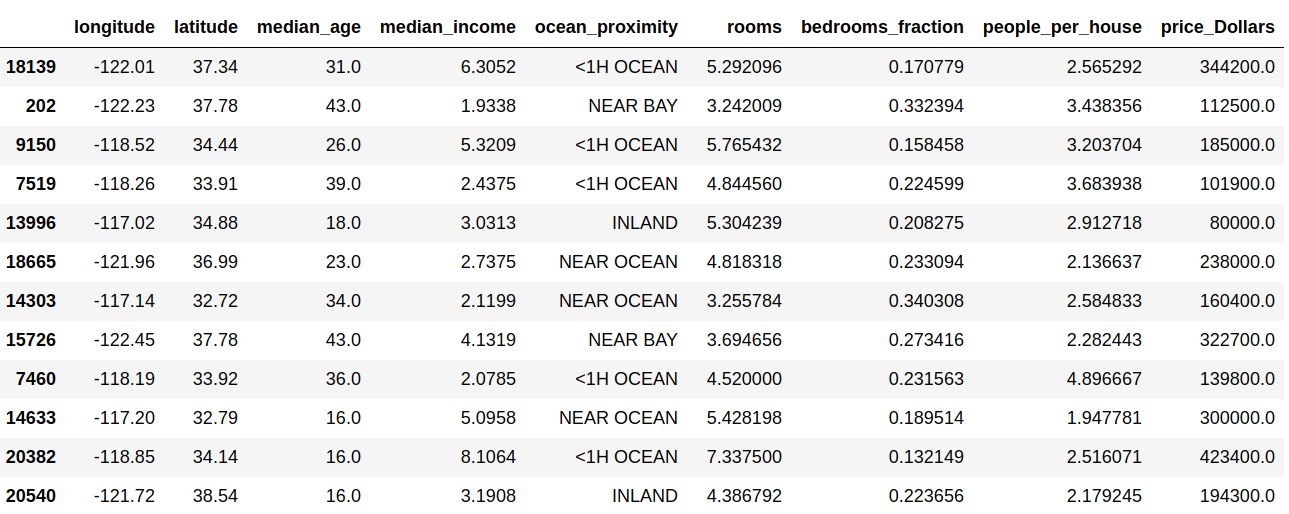
\includegraphics[scale=0.2]{housing_data.png}
\end{center}
\end{frame}

\begin{frame}[t]
\frametitle{Examples of Machine Learning}
\textcolor{orange2}{\textbf{Movie Ratings}}

Predict how a user would rate a movie.

\pause

\medskip

Each user is modelled as a vector of attributes:
\begin{itemize}
    \item likes comedy?  
    \item likes block-busters?
    \item likes sci-fi?
    \item likes a specific actor?
    \item $\ldots$
\end{itemize}

\pause

How would the user rate a given movie on a scale from $1$ to $10$?

\bigskip

\textbf{Data}
\begin{itemize}
    \item Data on how other users rated the given movie. 
\end{itemize}
\end{frame}


\begin{frame}[t]
\frametitle{Components of the Learning Problem}

\textbf{Formalization}

\begin{itemize}
    \item \textbf{Input:} $\vect{x}$ (applicant information)

    \pause

    \item \textbf{Output:} $y$ (good/bad customer)
    
    \pause

    \item \textbf{Target function:} $f \colon \calX \rightarrow \calY$ (ideal credit
    approval formula)
    
    \pause

    \item \textbf{Data:} $(\vect{x}^{(1)}, y^{(1)}), \ldots, (\vect{x}^{(m)},
    y^{(m)})$ (historical records)
    
    \pause

    \item \textbf{Hypothesis:} $h \colon \calX \rightarrow \calY$ (formula to be used)
\end{itemize} 
\end{frame}

\begin{frame}[t]
\frametitle{The Learning Problem}
\begin{center}
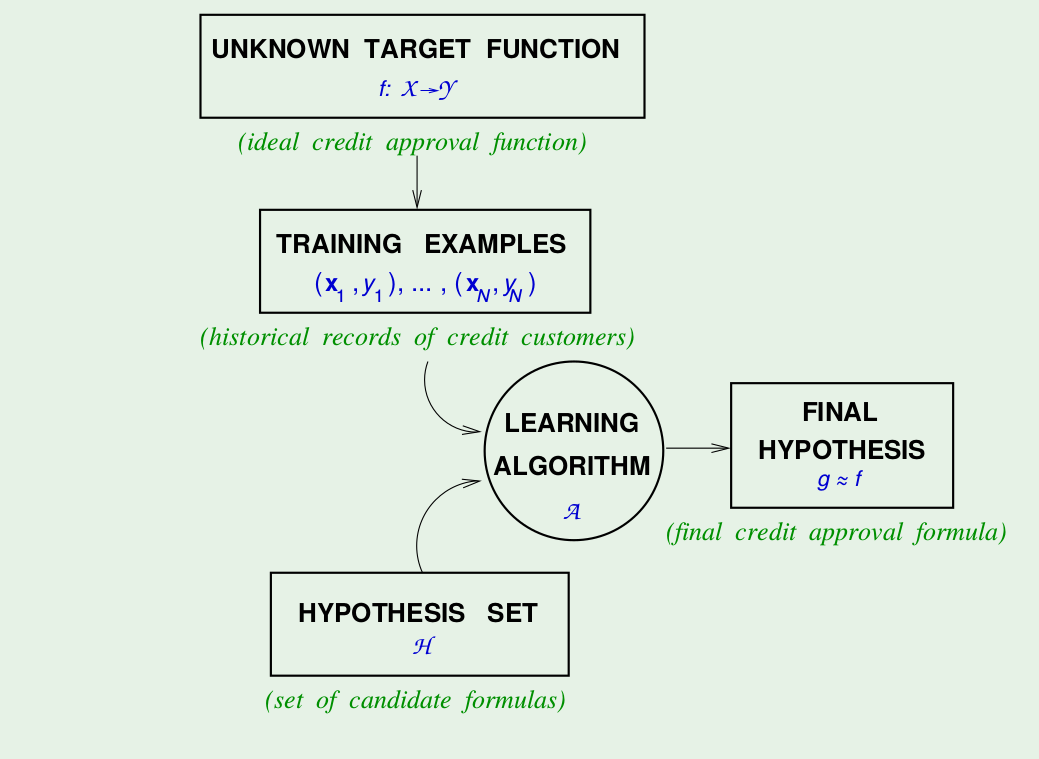
\includegraphics[scale=0.25]{the_learning_problem.png}
\end{center}
\end{frame}

\begin{frame}[t]
\frametitle{Solution Components}
Two solution components:
\begin{itemize}
    \item The Hypothesis Set $\cal{H}$
    \item The Learning Algorithm
\end{itemize}

Together, they are referred to as the \textbf{learning model}.

\pause

\bigskip

Why specify a hypothesis set?
\begin{itemize}
    \item This is what is generally done: you choose a linear model, 
    or an SVM or a neural network

    \item Important for developing a theory of learning 
\end{itemize}
\end{frame}

\begin{frame}[t]
\frametitle{Hypotheses Sets and Learning Algorithms}
\textbf{Examples}

\begin{center}
\begin{tabular}{ll}
\emph{Hypothesis Set} & \emph{Learning Algorithm} \\ \hline
Linear Regression & Gradient Descent \\
Neural Networks & Back Propagation \\
SVM & Quadratic Programming \\
Mixture of Gaussians Model & EM Algorithm \\
\end{tabular}
\end{center}
\end{frame}

\begin{frame}[t]
\frametitle{The Perceptron: A Simple Hypothesis Set}
For input $\vect{x} = (x_1, \ldots, x_n)$, the customer attributes,
\begin{align*}
\text{Approve credit if } & \sum_{i = 1}^{n} w_i x_i >    \text{ threshold} \\
\text{Deny credit if }    & \sum_{i = 1}^{n} w_i x_i \leq \text{ threshold}. \\
\end{align*}

This linear formula $g \in \cal{H}$ can be written as :
\[
    g(\vect{x}) = \sign \left (\sum_{i=1}^{n} w_i x_i - \text{ threshold} \right )
\]
\end{frame}

\begin{frame}[t]
\frametitle{The Perceptron: A Simple Hypothesis Set}
\[
    g(\vect{x}) = \sign \left (\sum_{i=1}^{n} w_i x_i - \text{ threshold} \right )
\]
\end{frame}

\begin{frame}[t]
\frametitle{The Perceptron: A Simple Hypothesis Set}
\[
    g(\vect{x}) = \sign \left (\sum_{i=1}^{n} w_i x_i + w_0\right )
\]

\pause

Introduce an artificial coordinate $x_0 = 1$:
\[
     g(\vect{x}) = \sign \sum_{i=0}^{n} w_i x_i = \sign(\trans{\vect{w}} \cdot \vect{x})
\]

\pause

\begin{center}
    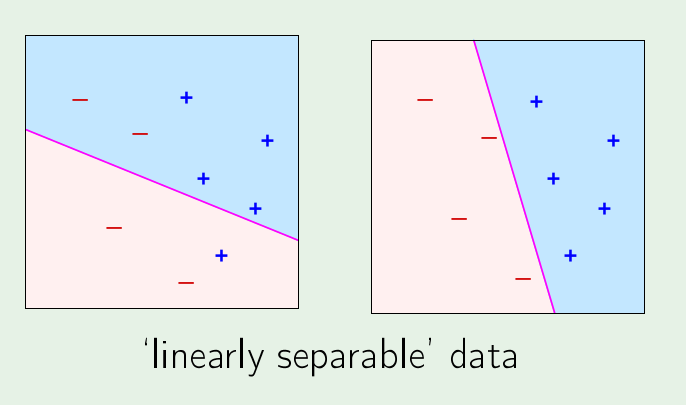
\includegraphics[scale=0.25]{linearly_separable_data.png}
\end{center}
\end{frame}

\begin{frame}[t]
\frametitle{The Perceptron Learning Algorithm (PLA)}
The perceptron implements 
\[g(\vect{x}) = \sign(\trans{\vect{w}} \cdot \vect{x})\]

\parbox[t]{5cm}{
Given a training set: 
\[(\vect{x}^{(1)}, y^{(1)}), (\vect{x}^{(2)}, y^{(2)}), \ldots, (\vect{x}^{(m)},
y^{(m)})\]
pick a \textbf{misclassified} point:
\[
    \sign (\trans{\vect{w}} \vect{x}^{(k)}) \neq y^{(k)}
\]
and update the weight vector:
\[
    \vect{w}_{\text{new}} \leftarrow \vect{w}_{\text{old}} + y^{(k)} \vect{x}^{(k)}
\]
} 
\hfill
\parbox[t]{5cm}{
\begin{center}
    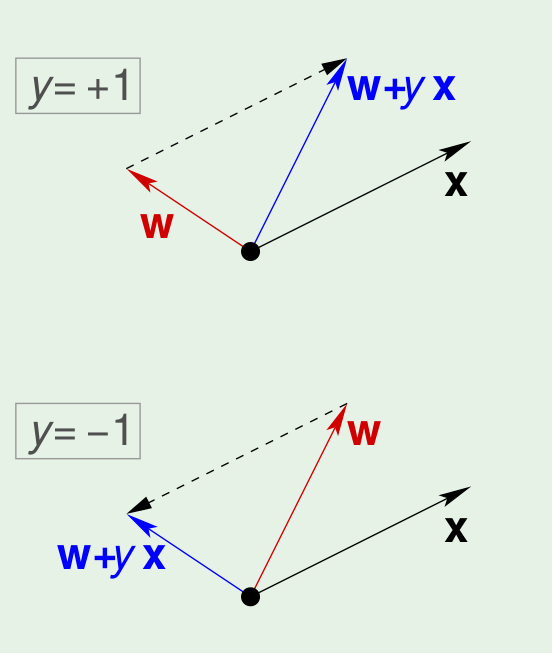
\includegraphics[scale=0.20]{PLA.png}
\end{center}
}
\end{frame}

\begin{frame}[t]
\frametitle{Iterations of PLA}
\parbox[t]{7cm}{
    \begin{itemize}
        \item One iteration of the PLA:
            \[ \vect{w}_{\text{new}} \leftarrow \vect{w}_{\text{old}} + y \vect{x}\]
        where $(\vect{x}, y)$ is a misclassified point.

        \item On iteration $i = 1, 2, 3, \ldots$, pick a misclassified point from 
            \[(\vect{x}^{(1)}, y^{(1)}), (\vect{x}^{(2)}, y^{(2)}), \ldots,
            (\vect{x}^{(m)}, y^{(m)})\]
        and run a PLA iteration on it. 
    \end{itemize}
}
\hfill
\parbox[t]{4cm}{
\begin{center}
    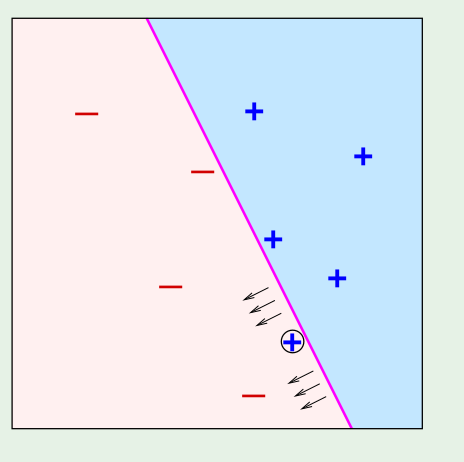
\includegraphics[scale=0.20]{PLA_iterations.png}
\end{center}
}

\begin{theorem}[Convergence]
If the data is linearly separable then the PLA will find a set of weights $\vect{w}$
that correctly classifies the training examples in a finite number of steps. 
\end{theorem}
\end{frame}

\begin{frame}[t]
\frametitle{Types of Learning}
\begin{itemize}
    \item Supervised Learning
    \item Unsupervised Learning
    \item Reinforced Learning 
\end{itemize}
\end{frame}

\begin{frame}[t]
\frametitle{Supervised Learning}
\begin{center}
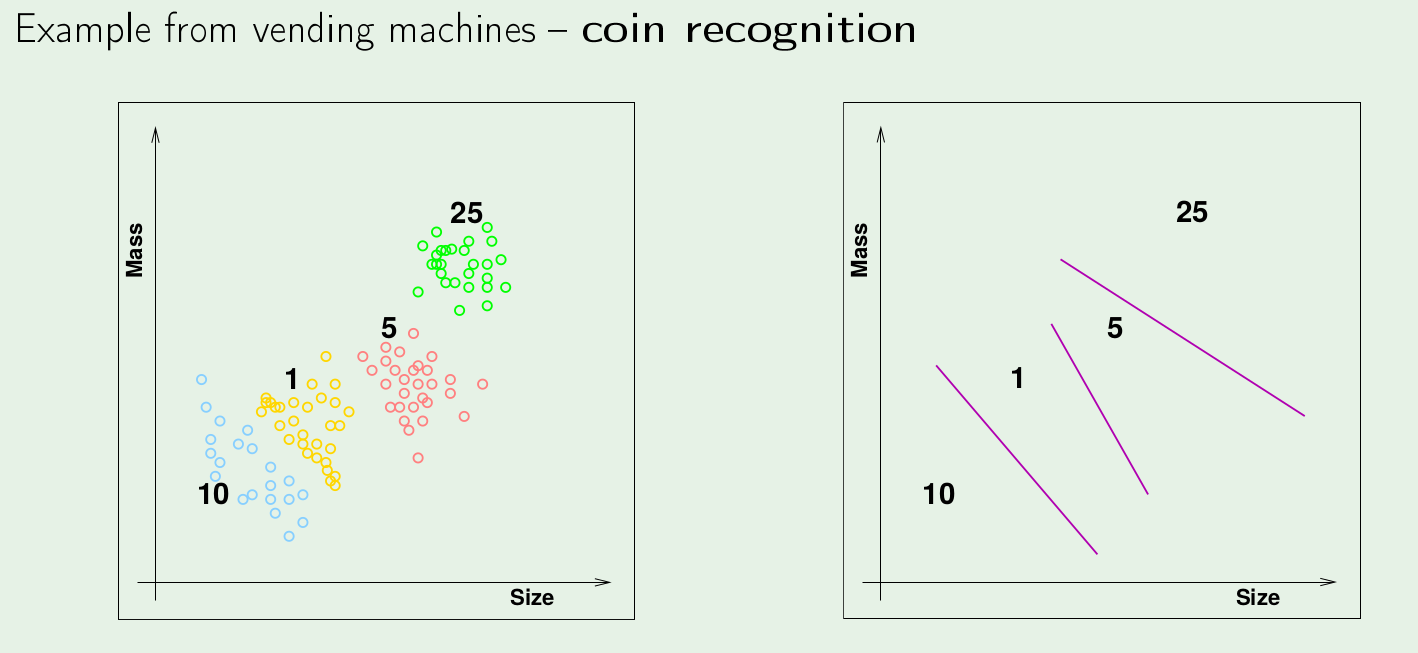
\includegraphics[scale=0.22]{supervised_learning.png}
\end{center}
\end{frame}

\begin{frame}[t]
\frametitle{Unsupervised Learning}
\begin{center}
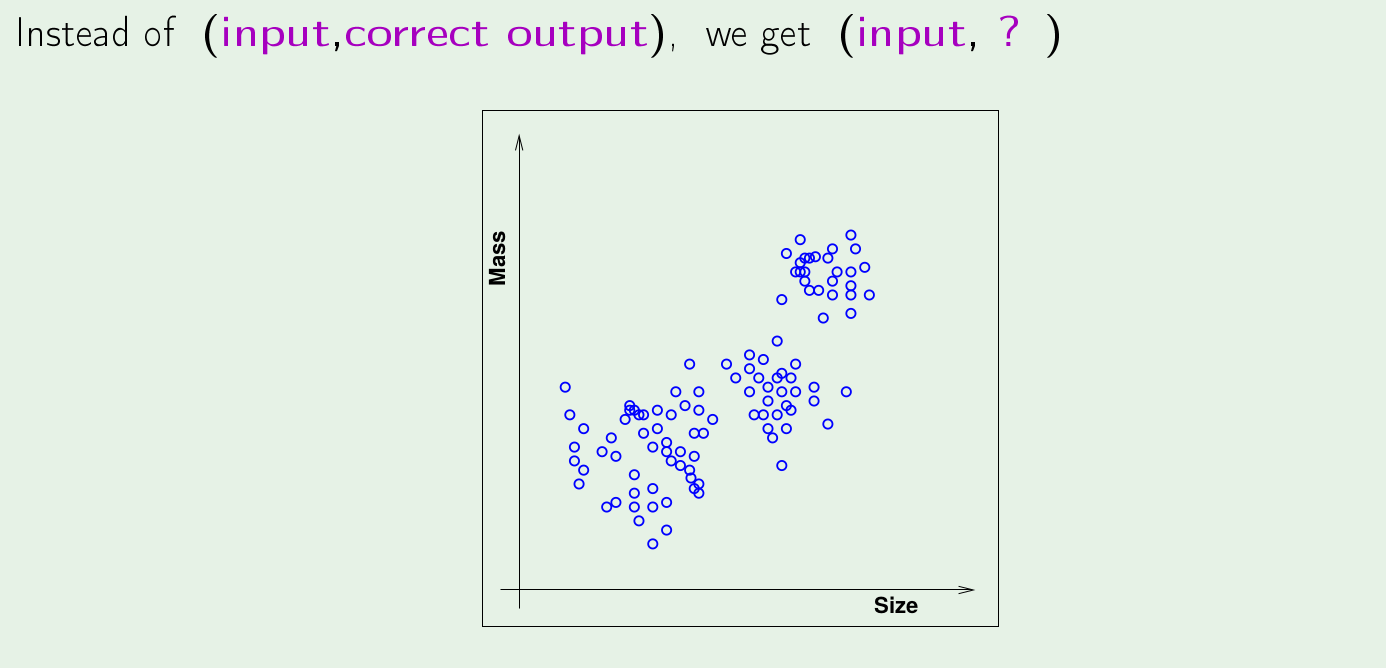
\includegraphics[scale=0.22]{unsupervised_learning.png}
\end{center}
\end{frame}

\begin{frame}[t]
\frametitle{Reinforced Learning}
\begin{center}
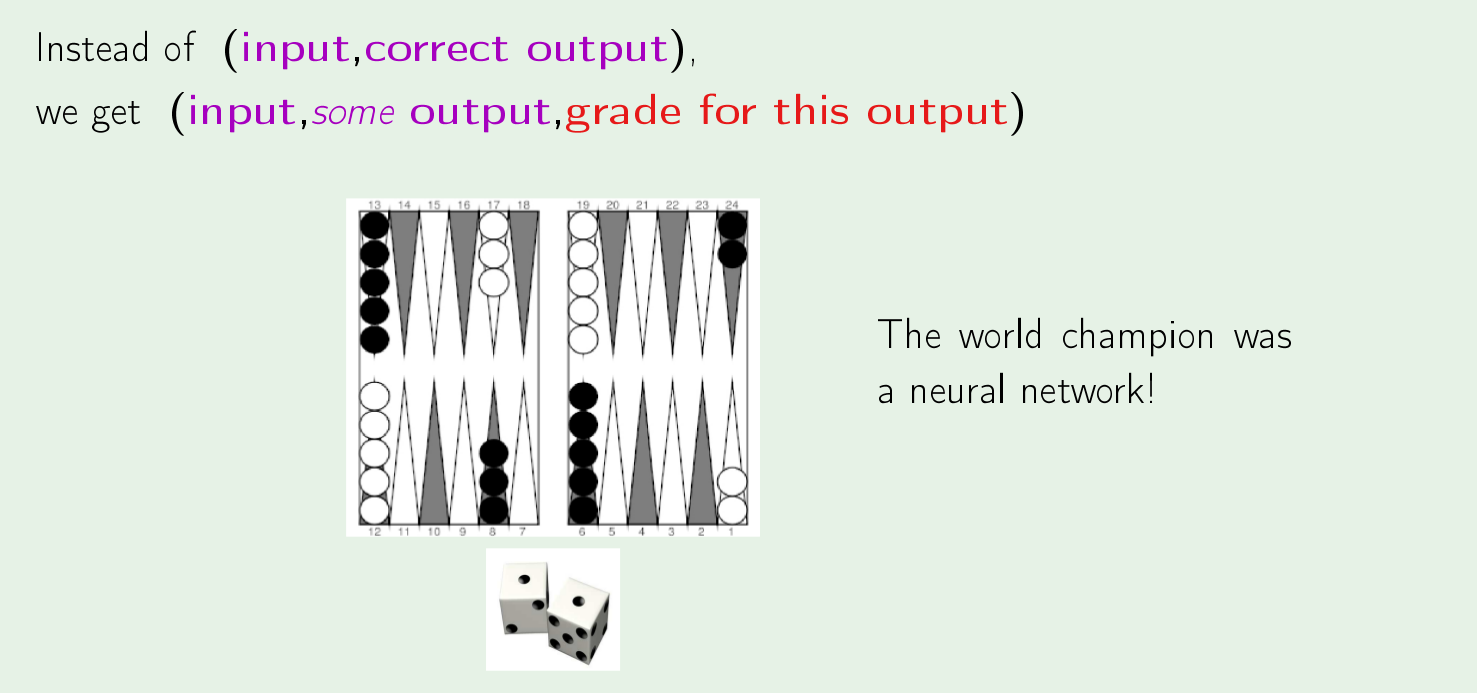
\includegraphics[scale=0.22]{reinforced_learning.png}
\end{center}
\end{frame}

\end{document}
